\documentclass[conference]{IEEEtran}
\IEEEoverridecommandlockouts
% The preceding line is only needed to identify funding in the first footnote. If that is unneeded, please comment it out.
\usepackage{cite}
\usepackage{amsmath,amssymb,amsfonts}
\usepackage{algorithmic}
\usepackage{graphicx}
\usepackage{textcomp}
\usepackage{xcolor}
\usepackage{booktabs}
\usepackage{soul}
\usepackage{amsmath}
\usepackage{url}
\def\BibTeX{{\rm B\kern-.05em{\sc i\kern-.025em b}\kern-.08em
    T\kern-.1667em\lower.7ex\hbox{E}\kern-.125emX}}

\graphicspath{ {./images/} }

\begin{document}

\title{Integrating Logical Dependencies in Software Clustering: A case of study on Apache Ant}

\author{\IEEEauthorblockN{1\textsuperscript{st} Adelina Stana}
\IEEEauthorblockA{\textit{Computer Science and Engineering Department} \\
\textit{"Politehnica" University of Timisoara}\\
 Timişoara, România \\
stana.adelina.diana@gmail.com }
\and
\IEEEauthorblockN{2\textsuperscript{nd} Ioana Sora}
\IEEEauthorblockA{\textit{Computer Science and Engineering Department} \\
\textit{"Politehnica" University of Timisoara}\\
 Timişoara, România \\
ioana.sora@cs.upt.ro}
}

\maketitle

\begin{abstract}
Extracted code co-changes from versioning systems have multiple applications across numerous fields, including fault detection, software reconstruction, key class identification, among others. This paper will focus on the influence of code co-changes on software clustering. Specifically, we will analyze their impact on the clustering solution of Apache Ant in order to assess whether co-changes usage enhances the quality of the obtained solution.
\end{abstract}

\begin{IEEEkeywords}
logical dependencies, logical coupling, mining software repositories, code co-change; co-changing entities, software evolution, clustering
\end{IEEEkeywords}

\section{Introduction}

The software architecture helps developers in gaining a better understanding of the system and its expected behavior. Additionally, it is also of great help in change management. By knowing the existing system architecture, project managers can assess whether a requested change can be easily implemented or not.

Architecture reconstruction appears in contexts where a software system lacks documentation entirely, or where the documentation hasn't been updated to reflect changes in the system. 

Previous research has revealed that dependencies extracted from versioning systems are distinct from those extracted from code, implying that using them could enhance our understanding of the system \cite{DBLP:conf/issre/OlivaG15}, \cite{DBLP:journals/jss/AjienkaC17}, \cite{Oliva:2011:ISL:2067853.2068086}.

We intend to use dependencies obtained from the versioning system to enhance the results of clustering methods that previously relied solely on connections extracted from code. 

To evaluate the results, we will initially create a clustering solution based on structural dependencies alone. Next, we will incorporate dependencies extracted from the versioning system with the structural dependencies to produce a second clustering solution. Lastly, we will construct a clustering solution that relies entirely on logical dependencies, and we will compare all three solutions obtained.


\section{Logical dependencies}
\label{ld_def}

During development processes, numerous software entities are changed. It has been observed that entities changing together are not only those with structural relationships but also include entities that are functionally dependent on one another. This functional dependency, however, cannot be observed by examining the code.

\begin{figure}
\centering
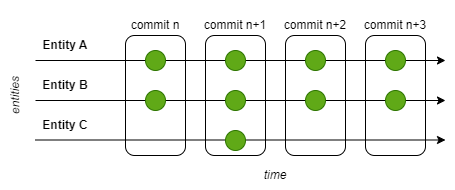
\includegraphics[scale=0.6]{dependencies.png}
\caption{Overview on updates of different entities}
\label{fig:dependencies}
\centering
\end{figure}

This type of entities, that consistently change together throughout development activities, are called logical dependencies or coupling. This concept was initially introduced by Gall et al. \cite{Gall:1998:DLC:850947.853338} and has numerous fields of application.

A problem with dependencies extracted from the versioning system is their potential to become excessively numerous. This often results from commits that contain numerous files, thereby generating thousands of dependencies from a single commit. Additionally, the reliability of co-changes is another problem; certain entities may only change together once throughout the entire versioning history, making them less reliable than entities that change together hundreds of times, for instance. Figure \ref{fig:dependencies} ilustrates this scenario.

Previous research uses two known metrics in order to solve this problems: \textit{support} and \textit{confidence}. Given a dependency where $A \rightarrow B$, the support metric measures the frequency of updates that two entities share within the versioning system. The confidence metric calculates the proportion of updates between two entities relative to the total updates of the antecedent (A) or consequent (B) entity \cite{DBLP:conf/issre/OlivaG15}, \cite{DBLP:journals/jss/AjienkaC17}, \cite{Zimmermann:2004:MVH:998675.999460}.


In our previous research, we focused on identifying metrics that enhance the reliability of dependencies extracted from the versioning system \cite{saci19}, \cite{enase19}. One of the metrics is the \textit{commit size metric}, which involves extracting dependencies from commits that do not exceed a specific commit size limit, thereby reducing the possibility of extracting an overly large number of dependencies. Additionally, we developed the strength metric, which serves as a refinement of the more known \textit{confidence metric} \cite{articlekeyclass23}.


The strength metric was developed to obtain a better reflection of the system and its values. For instance, when using the confidence metric, two entities that update together only once will have the highest possible score on the confidence metric, a result that is not desirable. On the other hand, entities that undergo hundreds of updates together, and even more updates with other entities, will receive a lower confidence metric score. Thus, the confidence metric will favor entities that update less and always together.

 The strength metric is calculated by multiplying the confidence metric value with a system factor, which is determined by the average number of updates for all entities in the system. In this way, a very high confidence score resulting from only a few updates will be adjusted downwards, while a low confidence score that is based on a big number of updates will be increased.

The confidence metric score ranges from 0 to 1, with 1 representing the best value. On the other hand, the strength metric ranges from 0 to 100, where 100 represents the best possible score.

Co-changes that meet both the commit size metric threshold and the strength metric threshold are referred to as \textit{logical dependencies}.

\section{Related work}

There are numerous applications of co-changes extracted from version control systems. Prajapati et al. used structural dependencies, co-changes, and lexical dependencies to enhance system modularization. Benkoczi et al. analyze how a system's modularity evolves over time using only co-change history \cite{10.1145/3196398.3196409}, by utilizing two metrics based on a weighted design structure matrix.

Anshu et al. analyze how co-changes impact the packaging restructuring \cite{clusters-cochange}, Silva et al. generated co-change clusters based on the versioning system information \cite{article-cochangem}.


The Modularization Quality (MQ) metric, as defined by Mitchell and Mancoridis \cite{mqmetric}, \cite{mqmetric2}, is extensively utilized to assess the results of clustering techniques. While it is primarily applied to clusters formed from structural dependencies \cite{Bunch1},\cite{Bunch2},\cite{Bunch3}, it also for evaluating clusters derived from other types of dependencies \cite{clustering-ld-lexical}.


\section{Method}
\label{method}

To obtain the logical dependencies for further use, we will use the same Python tool developed in our previous research \cite{articlekeyclass23}. This tool retrieves all necessary data from GitHub \cite{ApacheAntGitHub} using git commands and then processes it. 
The initial phase involves applying a commit size filter to exclude all commits that involve changes to more than 10 files. Following, the tool creates dependencies based on these commits, establishing a dependency link between each entity in a modified file and all entities in other files modified by the same commit. 

Next, the tool calculates the strength metric as described in chapter \ref{ld_def}. It then filters out any dependencies falling below the set strength metric threshold. For our experiments, we initiated with a strength metric threshold of 10, incrementing in steps of 10 up to 100 (the maximum value for the metric). Finally, we exported the results in comma separated values format file (.csv). The above described workflow is illustrated in figure \ref{fig:extraction}.


\begin{figure}
\centering
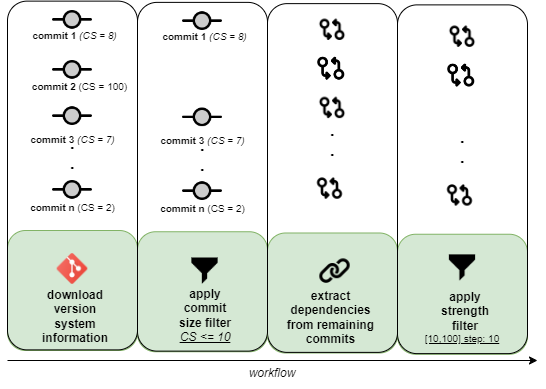
\includegraphics[width=\columnwidth]{dependencies-export.png}
\caption{Logical depenedencies extraction workflow}
\label{fig:extraction}
\centering
\end{figure}

Following the generation of logical dependencies, we integrate them into software clustering techniques. For this, a Python script was developed to extract both structural and logical dependencies from their respective files, forming a dependency matrix. This matrix is used as the input for the Minimum Spanning Tree (MST) and Louvain Clustering algorithms. The resulting clustering solution is then evaluated using the Modularity Quality (MQ) metric \cite{mqmetric}.

\subsection{Clustering algorithms: MST Clustering}
Minimum Spanning Tree Clustering is a hierarchical clustering method based on the construction of a minimum spanning tree from the weighted graph formed by the data connections of the system \cite{mst_clustering}.


\subsection{Clustering algorithms: Louvain Clustering}
Louvain Clustering is a community detection algorithm designed for finding clusters or communities in complex networks. The Louvain method involves a greedy algorithm that moves nodes between clusters to obtain clusters that are highly interconnected \cite{louvain_clustering}.

In order to compare the clustering solutions and their asociated MQ metric, we generated clustering solutions in three scenarios: the first one by using only structural dependencies, the second one by using only logical dependencies and the third one by using logical and structural dependencies to populate the dependency matrix that is further used in the cluster generation. The third scenario workflow is ilustrated in the figure \ref{fig:clustering-gen}.

To generate and compare the clustering solutions and their corresponding Modularity Quality (MQ) metric, we created clustering solutions for three distinct scenarios: the first scenario utilizes solely structural dependencies, the second exclusively employs logical dependencies, and the third combines both logical and structural dependencies to fill the dependency matrix, which is then utilized in generating the clusters. The process for the third scenario is depicted in Figure \ref{fig:clustering-gen}.

\begin{figure}
\centering
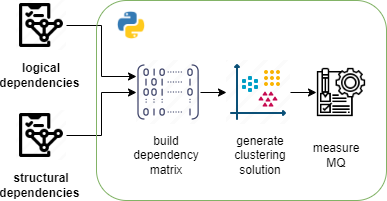
\includegraphics[width=\columnwidth]{clustering-generation.png}
\caption{Clustering solution creation process diagram}
\label{fig:clustering-gen}
\centering
\end{figure}


\section{Results}
\label{results}

The results of the scenarios mentioned in chapter \ref{method} are presented in table \ref{tab:clustering-results1} and \ref{tab:clustering-results2}.

\begin{table}[htbp]
  \centering
  \caption{Comparison of Louvain and MST clustering results for LD}
  \label{tab:clustering-results1}
  \begin{tabular}{lc|cc|cc}
    \toprule
    \textbf{Dataset} & \textbf{Entities} & \multicolumn{2}{c}{\textbf{Cluster count}} & \multicolumn{2}{c}{\textbf{MQ metric}} \\
    & \textbf{Count} & \textbf{Louvain} & \textbf{MST} & \textbf{Louvain} & \textbf{MST} \\
    \midrule
    SD only & 517 & 14 & 228 & 0.085 & 0.084 \\
    LD strength 10\% & 517 & 272 & 353 & 0.047 & 0.031 \\
    LD strength 20\% & 517 & 355 & 360 & 0.04 & 0.037 \\
    LD strength 30\% & 517 & 387 & 404 & 0.036 & 0.033 \\
    LD strength 40\% & 517 & 405 & 413 & 0.034 & 0.033 \\
    LD strength 50\% & 517 & 414 & 422 & 0.03 & 0.029 \\
    LD strength 60\% & 517 & 431 & 439 & 0.029 & 0.027 \\
    LD strength 70\% & 517 & 443 & 444 & 0.027 & 0.026 \\
    LD strength 80\% & 517 & 454 & 460 & 0.024 & 0.022 \\
    LD strength 90\% & 517 & 462 & 463 & 0.021 & 0.021 \\
    LD strength 100\% & 517 & 472 & 480 & 0.019 & 0.016 \\
    \bottomrule
  \end{tabular}
\end{table}



\begin{table}[htbp]
  \centering
  \caption{Comparison of Louvain and MST clustering results for LD combined with SD}
  \label{tab:clustering-results2}
  \begin{tabular}{lc|cc|cc}
    \toprule
    \textbf{Dataset} & \textbf{Entities} & \multicolumn{2}{c}{\textbf{Cluster count}} & \multicolumn{2}{c}{\textbf{MQ metric}} \\
    & \textbf{Count} & \textbf{Louvain} & \textbf{MST} & \textbf{Louvain} & \textbf{MST} \\
    \midrule
    SD only & 517 & 14 & 228 & 0.085 & 0.084 \\
    SD  LD strength 10\% & 517 & 15 & 74 & 0.087 & \underline{0.054} \\
    SD  LD strength 20\% & 517 & 13 & 8 & 0.071 & \underline{0.059} \\
    SD  LD strength 30\% & 517 & 13 & 14 & 0.071 & \underline{0.083} \\
    SD  LD strength 40\% & 517 & 13 & 8 & 0.071 & 0.109 \\
    SD  LD strength 50\% & 517 & 13 & 8 & 0.071 & 0.109 \\
    SD  LD strength 60\% & 517 & 13 & 8 & 0.071 & 0.109 \\
    SD  LD strength 70\% & 517 & 13 & 10 & 0.071 & 0.155 \\
    SD  LD strength 80\% & 517 & 13 & 6 & 0.071 & 0.177 \\
    SD  LD strength 90\% & 517 & 13 & 2 & 0.071 & 0.129 \\
    SD  LD strength 100\% & 517 & 13 & 8 & 0.072 & 0.166 \\
    \bottomrule
  \end{tabular}
\end{table}






\section{Discussion}
\label{discussion}

Based on the results from table \ref{tab:clustering-results2}, we can observe that the combined approach of structural dependencies and logical dependencies gives a Modularity Quality (MQ) metric of 0.071, which is an improvement over the 0.085 MQ metric obtained when considering only structural dependencies. 

Next, we will examine the clustering solutions obtained only from structural dependencies, in comparison to the clustering solution derived from incorporating both structural and logical dependencies, filtered with a threshold of 20\% for strength.

The entities listed below are placed in different clusters when analyzed based on structural dependencies alone, compared with the analysis using both logical and structural dependencies: taskdefs.Available\$FileDir, taskdefs.Concat, taskdefs.Concat\$1, taskdefs.Concat\$MultiReader, taskdefs.Concat\$TextElement, taskdefs.Javadoc\$AccessType, util.WeakishReference, util.WeakishReference\$HardReference.

The placement of the Concat class and its inner classes (Concat\$1, Concat\$MultiReader, Concat\$TextElement) in a different cluster might be based on it's usage and purpose; according to the documentation : "This class contains the 'concat' task, used to concatenate a series of files into a single stream." \cite{ant_concat}. \ref{fig:cluster1}

\begin{figure}
\centering
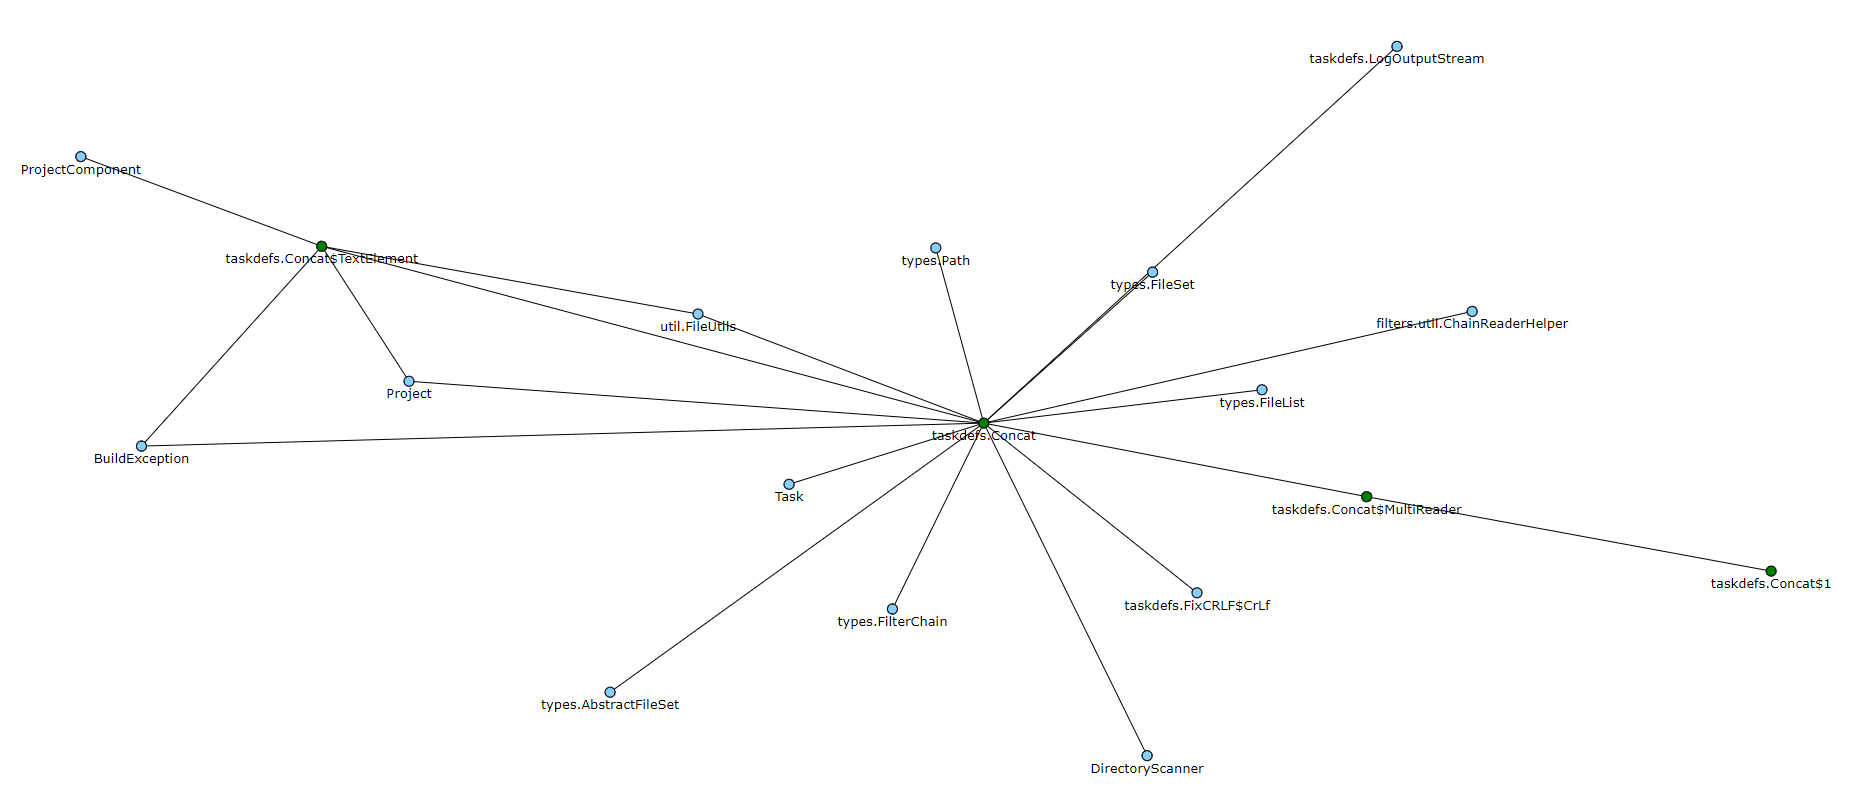
\includegraphics[width=\columnwidth]{cluster1.png}
\caption{Ant cluster}
\label{fig:cluster1}
\centering
\end{figure}

\section{Conclusion and Future work}

Based the outcomes detailed in Chapter \ref{results} and the analysis in Chapter \ref{discussion}, it is clear that incorporating logical dependencies improves the quality of clustering solutions. For our forthcoming work, we intend to conduct further experiments across various projects to validate these findings. Additionally, we will try to create a reference clustering solution for these projects, based on their code and documentation. We will then evaluate the clustering results against the reference solution by utilizing the MOJO metric for comparison \cite{mojo-tzerpos}.


\bibliographystyle{IEEEtran}
\bibliography{logicaldepd}

\end{document}
